\documentclass{beamer}

\usepackage{pgfpages}
\usepackage{caption}
\usepackage{listings}
\usepackage{amsmath}
\usepackage{makecell}
\setbeameroption{show notes on second screen}

\setbeamertemplate{caption}[numbered]
\setbeamerfont{note page}{size=\scriptsize}

\usetheme{Bergen}
\usecolortheme{beetle}

\mode<presentation>

\title{Perbandingan Algoritma \textit{Backtracking} dan Algoritma \textit{Hybrid Genetic} untuk Menyelesaikan Permainan Calcudoku}
\author{Michael Adrian \\ 2013730039 \\ \texttt{michaeladrian39@gmail.com}}
\institute{Program Studi Teknik Informatika \\ Fakultas Teknologi Informasi dan Sains \\ Universitas Katolik Parahyangan}
\date{20 Desember 2017}

\begin{document}

\begin{frame}
\titlepage
\end{frame}

\section{Dasar Teori}

\subsection{Calcudoku}

\begin{frame}
\frametitle{Calcudoku}
\begin{itemize}
\item Salah satu jenis permainan teka-teki aritmatika dan logika
\item Dikenal juga sebagai KenKen, KenDoku, atau Mathdoku
\end{itemize}
\end{frame}

\note{
Sebagai salah satu jenis permainan teka-teki aritmatika dan \textit{grid}, Calcudoku, atau dikenal juga sebagai KenKen, KenDoku, atau Mathdoku.
}

\begin{frame}
\frametitle{Aturan Permainan}
\begin{itemize}
\item Pemain diberikan sebuah \textit{grid} dengan ukuran \begin{math}n \times n\end{math}
\item \begin{math}n\end{math} biasanya antara 3 sampai dengan 9
\item \textit{Grid} ini harus diisi dengan angka 1 sampai dengan \begin{math}n\end{math}
\item Dalam setiap baris setiap angka hanya muncul sekali
\item Dalam setiap kolom setiap angka hanya muncul sekali
\item \textit{Grid} dibagi ke dalam \textit{cage}
\item \textit{Cage} adalah sekelompok sel yang dibatasi oleh garis yang lebih tebal daripada garis pembatas antar sel dengan angka tujuan dan operator yang telah ditentukan
\item Angka-angka dalam setiap \textit{cage} harus mencapai angka tujuan jika dihitung menggunakan operator yang telah ditentukan
\item Angka tujuan dan operasi yang telah ditentukan ditulis di sudut kiri atas \textit{cage}
\end{itemize}
\end{frame}

\note{
Seperti dalam Sudoku, dalam teka-teki ini, pemain diberikan sebuah \textit{grid} dengan ukuran \begin{math}n \times n\end{math}, dengan \begin{math}n\end{math} biasanya antara 3 sampai dengan 9. \textit{Grid} ini harus diisi dengan angka 1 sampai dengan \begin{math}n\end{math} sehingga dalam setiap baris setiap angka hanya muncul sekali, dalam setiap kolom setiap angka hanya muncul sekali. Perbedaannya dengan Sudoku adalah, Calcudoku dibagi ke dalam \textit{cage} (sekelompok sel yang dibatasi oleh garis yang lebih tebal daripada garis pembatas antar sel dengan angka tujuan dan operator yang telah ditentukan), dan angka-angka dalam setiap \textit{cage} harus mencapai angka tujuan jika dihitung menggunakan operator yang telah ditentukan. Angka tujuan dan operasi yang telah ditentukan ditulis di sudut kiri atas \textit{cage}.
}

\begin{frame}
\frametitle{Operator-Operator Matematika}
\begin{itemize}
\item Ada 5 kemungkinan operator:
	\begin{itemize}
	\item + (penjumlahan)
	\item - (pengurangan)
	\item \begin{math}\times\end{math} (perkalian)
	\item \begin{math}\div\end{math} (pembagian)
	\item = (sama dengan)
	\end{itemize}
\item Jika operasi matematika yang ditentukan adalah pengurangan atau pembagian, maka ukuruan \textit{cage} harus berukuran dua sel
\end{itemize}
\end{frame}

\note{
Ada lima kemungkinan operator:
\begin{enumerate}
\item +, sebuah operator \begin{math}n\end{math}-ary yang menandakan penjumlahan.
\item -, sebuah operator biner yang menandakan pengurangan.
\item \begin{math}\times\end{math}, sebuah operator  \begin{math}n\end{math}-ary yang menandakan perkalian.
\item \begin{math}\div\end{math} sebuah operator biner yang menandakan pembagian.
\item =, (simbol ini biasanya dihilangkan), sebuah operator uner yang menandakan persamaan.
\end{enumerate}
Jika operasi matematika yang ditentukan adalah pengurangan atau pembagian, maka ukuruan \textit{cage} harus berukuran dua sel. Pada beberapa versi dari teka-teki ini, hanya angka tujuan yang diberikan, dan pemain harus menebak operator dari setiap \textit{cage} untuk menyelesaikan teka-tekinya.
}

\begin{frame}
\frametitle{Contoh Permainan}
\begin{figure}
\centering
\captionsetup{justification=centering}
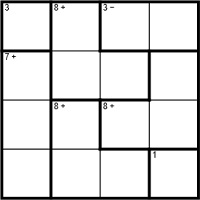
\includegraphics[scale=1]{Gambar/Backtracking1}
\caption[Contoh permainan teka-teki Calcudoku dengan ukuran \textit{grid} 4 x 4 yang belum diselesaikan. ]{Contoh permainan teka-teki dengan ukuran \textit{grid} 4 x 4 yang belum diselesaikan. }
\label{fig:backtracking1}
\end{figure}
\end{frame}

\begin{frame}
\frametitle{Contoh Solusi}
\begin{figure}
\centering
\captionsetup{justification=centering}
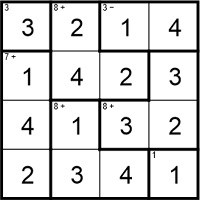
\includegraphics[scale=1]{Gambar/Backtracking2}
\caption[Solusi untuk permainan teka-teki Calcudoku yang diberikan pada Gambar~\ref{fig:backtracking1} ]{Solusi untuk permainan teka-teki Calcudoku yang diberikan pada Gambar~\ref{fig:backtracking1}. }
\label{fig:backtracking2}
\end{figure}
\end{frame}

\subsection{Algoritma \protect\textit{Backtracking}}

\begin{frame}
\frametitle{Algoritma \protect\textit{Backtracking}}
\begin{itemize}
\item Sebuah algoritma umum yang mencari solusi dengan mencoba salah satu dari beberapa pilihan, jika pilihan yang dipilih ternyata salah, komputasi dimulai lagi pada titik pilihan dan mencoba pilihan lainnya
\item Untuk bisa melacak kembali langkah-langkah yang telah dipilih, maka algoritma harus secara eksplisit menyimpan jejak dari setiap langkah yang sudah pernah dipilih, atau menggunakan rekursi (\textit{recursion})
\item Rekursi dipilih karena jauh lebih mudah daripada harus menyimpan jejak setiap langkah yang pernah dipilih
\item Hal ini menyebabkan algoritma ini biasanya berbasis DFS (\textit{Depth First Search})
\end{itemize}
\end{frame}

\note{
Algoritma \textit{backtracking} adalah sebuah algoritma umum yang mencari solusi dengan mencoba salah satu dari beberapa pilihan, jika pilihan yang dipilih ternyata salah, komputasi dimulai lagi pada titik pilihan dan mencoba pilihan lainnya. Untuk bisa melacak kembali langkah-langkah yang telah dipilih, maka algoritma harus secara eksplisit menyimpan jejak dari setiap langkah yang sudah pernah dipilih, atau menggunakan rekursi (\textit{recursion}). Rekursi dipilih karena jauh lebih mudah daripada harus menyimpan jejak setiap langkah yang pernah dipilih. Hal ini menyebabkan algoritma ini biasanya berbasis DFS (\textit{Depth First Search}).
}

\begin{frame}
\frametitle{Cara Kerja Algoritma \protect\textit{Backtracking} Secara Singkat}
\begin{itemize}
\item Singkatnya, langkah-langkah dasar dari implementasi algoritma \textit{backtracking} dapat dijelaskan sebagai berikut:
\begin{enumerate}
	\item Carilah sel pertama atau sel yang kosong di dalam \textit{grid}
	\item Isilah sel dengan sebuah angka dimulai dari 1 sampai \begin{math}n\end{math} sampai sebuah angka yang berlaku (\textit{valid}) ditemukan atau sampai angka sudah melebihi \begin{math}n\end{math}
	\item Jika angka untuk sel berlaku, ulangi langkah 1 dan 2
	\item Jika angka untuk sel sudah melebihi \begin{math}n\end{math} dan tidak ada angka dari 1 sampai \begin{math}n\end{math} yang berlaku untuk sel tersebut, mundur ke sel sebelumnya dan cobalah kemungkinan angka berikutnya yang berlaku untul sel tersebut
	\item Jika tidak ada lagi sel yang kosong, solusi sudah ditemukan
	\end{enumerate}
\end{itemize}
\end{frame}

\note{
Singkatnya, langkah-langkah dasar dari implementasi algoritma \textit{backtracking} dapat dijelaskan sebagai berikut ~\cite{fahda:16:backtracking}:
\begin{enumerate}
\item Carilah sel pertama atau sel yang kosong di dalam \textit{grid}.
\item Isilah sel dengan sebuah angka dimulai dari 1 sampai \begin{math}n\end{math} sampai sebuah angka yang berlaku (\textit{valid}) ditemukan atau sampai angka sudah melebihi \begin{math}n\end{math}.
\item Jika angka untuk sel berlaku, ulangi langkah 1 dan 2.
\item Jika angka untuk sel sudah melebihi \begin{math}n\end{math} dan tidak ada angka dari 1 sampai \begin{math}n\end{math} yang berlaku untuk sel tersebut, mundur ke sel sebelumnya dan cobalah kemungkinan angka berikutnya yang berlaku untul sel tersebut.
\item Jika tidak ada lagi sel yang kosong, solusi sudah ditemukan.
\end{enumerate}
}

\subsection{Algoritma \protect\textit{Hybrid Genetic}}

\begin{frame}
\frametitle{Algoritma \textit{Hybrid Genetic}}
\begin{itemize}
\item Dalam kasus ini, algoritma \textit{hybrid genetic} adalah gabungan dari algoritma \textit{rule based} dan algoritma genetik
\item Algoritma \textit{rule based} akan dijalankan sampai pada titik dimana algoritma tidak bisa menyelesaikan permainan teka-teki Calcudoku
\item Jika algoritma sudah tidak bisa menyelesaikan permainan, maka algoritma genetik akan mulai dijalankan
\end{itemize}
\end{frame}

\note{
Dalam kasus ini, algoritma ini gabungan dari algoritma \textit{rule based} dan algoritma genetik. Algoritma \textit{rule based} akan dijalankan sampai pada titik dimana algoritma tidak bisa menyelesaikan permainan teka-teki Calcudoku. Jika algoritma sudah tidak bisa menyelesaikan permainan, maka algoritma genetik akan mulai dijalankan.
}

\begin{frame}
\frametitle{Algoritma \textit{Rule Based}}
\begin{itemize}
\item Sebuah algoritma berbasis aturan logika untuk menyelesaikan teka-teki Sudoku dan variasinya, termasuk Calcudoku
\item Beberapa aturan logika yang digunakan dalam algoritma ini adalah:
	\begin{itemize}
 	\item \textit{Single square rule}
	\item \textit{Naked subset rule}
	\item \textit{Hidden single rule}
	\item \textit{Killer combination}
	\end{itemize}
\end{itemize}
\end{frame}

\note{
Algoritma \textit{rule based} adalah sebuah algoritma berbasis aturan logika untuk menyelesaikan teka-teki Sudoku dan variasinya, termasuk Calcudoku. Menurut Johanna, Lukas, dan Saputra, beberapa aturan logika yang digunakan dalam algoritma ini adalah \textit{single square rule}, \textit{naked subset rule}, \textit{hidden single rule}, \textit{evil twin rule}, \textit{killer combination}, dan \textit{X-wing} ~\cite{johanna:12:hybrid}.
}

\begin{frame}
\frametitle{Algoritma Genetik}
\begin{itemize}
\item Salah satu teknik heuristik \textit{Generate and Test} yang terinspirasi oleh sistem seleksi alam
\item Perpaduan dari bidang biologi dan ilmu komputer.
\item Algoritma ini memanipulasi informasi, biasanya disebut sebagai kromosom.
\end{itemize}
\end{frame}

\note{
Algoritma genetik adalah salah satu teknik heuristik \textit{Generate and Test} yang terinspirasi oleh sistem seleksi alam. Algoritma ini adalah perpaduan dari bidang biologi dan ilmu komputer. Algoritma ini memanipulasi informasi, biasanya disebut sebagai kromosom. 
}

\begin{frame}
\frametitle{Cara Kerja Algoritma Genetik}
\begin{itemize}
\item Cara kerja algoritma genetik adalah sebagai berikut:
\begin{enumerate}
\item Menentukan populasi kromosom kemungkinan jawaban awal
\item Membangkitkan populasi kemungkinan jawaban awal secara acak
\item Mengevaluasi fungsi objektif
\item Melakukan operasi terhadap kromosom menggunakan operator genetik (reproduksi, kawin silang, dan mutasi)
\item Ulangi langkah 3 dan 4 sampai mencapai kriteria untuk menghentikan algoritm.
\end{enumerate}
\end{itemize}
\end{frame}

\note{
Cara kerja algoritma genetik adalah sebagai berikut ~\cite{johanna:12:hybrid}:
	\begin{enumerate}
	\item Menentukan populasi kromosom kemungkinan jawaban awal.
	\item Membangkitkan populasi kemungkinan jawaban awal secara acak.
	\item Mengevaluasi fungsi objektif.
	\item Melakukan operasi terhadap kromosom menggunakan operator genetik (reproduksi, kawin silang, dan mutasi).
	\item Ulangi langkah 3 dan 4 sampai mencapai kriteria untuk menghentikan algoritma.
	\end{enumerate}
}

\begin{frame}
\frametitle{Cara Kerja Algoritma \textit{Hybrid Genetic}}
\begin{itemize}
\item Cara kerja algoritma \textit{hybrid genetic} adalah sebagai berikut:
	\begin{itemize}
	\item Masukkan teka-teki yang akan diselesaikan sebagai input.
	\item Program akan merepresentasikan input yang dimasukkan dalam format teka-teki.
	\item Program akan mencoba menyelesaikan teka-teki tersebut dengan menggunakan algoritma \textit{rule based} terlebih dahulu.
	\item Jika program berhasil menyelesaikan teka-teki tersebut dengan menggunakan algoritma \textit{rule based}, maka algoritma selesai.
	\item Jika program gagal dengan menggunakan algoritma \textit{rule based}, maka program akan mencoba menyelesaikan teka-teki tersebut dengan menggunakan algoritma genetik.
	\item Jika program berhasil menyelesaikan teka-teki tersebut dengan menggunakan algoritma genetik, maka algoritma selesai.
	\item Jika program gagal dalam menyelesaikan teka-teki tersebut setelah menggunakan algoritma genetik, artinya algoritma gagal dalam menyelesaikan teka-teki terseebut.
	\end{itemize}
\end{itemize}
\end{frame}

\note{
Cara kerja algoritma \textit{hybrid genetic} menurut Johanna, Lukas, dan Saputra adalah sebagai berikut ~\cite{johanna:12:hybrid}:
\begin{itemize}
\item Masukkan teka-teki yang akan diselesaikan sebagai input.
\item Program akan merepresentasikan input yang dimasukkan dalam format teka-teki.
\item Program akan mencoba menyelesaikan teka-teki tersebut dengan menggunakan algoritma \textit{rule based} terlebih dahulu.
\item Jika program berhasil menyelesaikan teka-teki tersebut dengan menggunakan algoritma \textit{rule based}, maka algoritma selesai.
\item Jika program gagal dengan menggunakan algoritma \textit{rule based}, maka program akan mencoba menyelesaikan teka-teki tersebut dengan menggunakan algoritma genetik.
\item Jika program berhasil menyelesaikan teka-teki tersebut dengan menggunakan algoritma genetik, maka algoritma selesai.
\item Jika program gagal dalam menyelesaikan teka-teki tersebut setelah menggunakan algoritma genetik, artinya algoritma gagal dalam menyelesaikan teka-teki terseebut.
\end{itemize}
}

\begin{frame}
\frametitle{Alur Cara Kerja Algoritma \textit{Hybrid Genetic}}
\begin{figure}
\centering
\captionsetup{justification=centering}
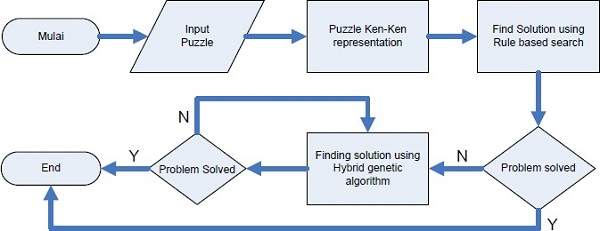
\includegraphics[scale=0.5]{Gambar/HybridGenetic7}
\caption[Alur penyelesaian permainan teka-teki Calcudoku dengan menggunakan algoritma \textit{hybrid genetic} ~\cite{johanna:12:hybrid}]{Alur penyelesaian permainan teka-teki Calcudoku dengan menggunakan algoritma \textit{hybrid genetic}}
\label{fig:hybrid7}
\end{figure}
\begin{itemize}
\item Alur (\textit{flow chart}) penyelesaian permainan teka-teki Calcudoku dengan menggunakan algoritma \textit{hybrid genetic} dapat dilihat di Gambar~\ref{fig:hybrid7}.
\end{itemize}
\end{frame}

\note{
Alur (\textit{flow chart}) penyelesaian permainan teka-teki Calcudoku dengan menggunakan algoritma \textit{hybrid genetic} dapat dilihat di Gambar~\ref{fig:hybrid7}.
}

\section{Analisis}

\begin{frame}
\frametitle{Analisis Perangkat Lunak}
\begin{itemize}
\item Perangkat lunak ini akan menerima masukan dalam bentuk \textit{file} yang berisi:
	\begin{enumerate}
	\item Ukuran \textit{grid}
	\item Jumlah \textit{cage}
	\item Matriks \textit{cage assignment}
	\item Matriks \textit{cage objectives}
\end{enumerate}
\item Perangkat lunak ini akan menghasilkan keluaran berupa GUI permainan teka-teki Calcudoku berdasarkan isi \textit{file} yang di-\textit{load} oleh pengguna.
\item Permainan ini dapat diselesaikan oleh pengguna, atau menggunakan salah satu dari dua \textit{solver} yang disediakan. Kedua \textit{solver} tersebut yaitu:
	\begin{enumerate}
	\item Algoritma \textit{backtracking}, dan
	\item Algoritma \textit{hybrid genetic}.
	\end{enumerate}
\end{itemize}
\end{frame}

\note{
Perangkat lunak ini akan menerima masukan dalam bentuk \textit{file} yang berisi:

\begin{enumerate}
\item Ukuran \textit{grid}.
\item Jumlah \textit{cage}.
\item Matriks \textit{cage assignment}, yang merepresentasikan posisi dari setiap \textit{cage} dalam \textit{grid}.
\item Matriks \textit{cage objectives}, yang berisikan angka tujuan dan operasi matematika yang telah ditentukan untuk setiap \textit{cage}.
\end{enumerate}

Perangkat lunak ini akan menghasilkan keluaran berupa antarmuka grafis permainan teka-teki Calcudoku berdasarkan isi \textit{file} yang di-\textit{load} oleh pengguna.

Permainan ini dapat diselesaikan oleh pengguna dengan usahanya sendiri, atau menggunakan salah satu dari dua \textit{solver} yang disediakan. Kedua \textit{solver} tersebut yaitu:

\begin{enumerate}
\item Algoritma \textit{backtracking}, dan
\item Algoritma \textit{hybrid genetic}.
\end{enumerate}
}

\begin{frame}
\frametitle{Diagram \textit{Use Case}}
\begin{itemize}
\item Diagram \textit{use case} adalah diagram yang menggambarkan interaksi antara sistem (perangkat lunak) dengan pengguna.
\item Skenario-skenario yang dapat dilakukan oleh pengguna adalah:
	\begin{enumerate}
	\item Membuka file masukan.
	\item Memilih salah satu dari dua \textit{solver} yang disediakan.
	\item Me-\textit{reset} permainan.
	\item Memeriksa permainan.
	\item Menutup \textit{file} masukan.
	\item Menyelesaikan permainan dengan usahanya sendiri.
	\item Mengatur nilai dari parameter-parameter untuk algoritma genetik.
	\end{enumerate}
\item Diagram \textit{use case} berdasarkan skenario-skenario tersebut dapat dilihat pada Gambar~\ref{fig:analisisusecase}.
\end{itemize}
\end{frame}

\note{
Diagram \textit{use case} adalah diagram yang menggambarkan interaksi antara sistem (perangkat lunak) dengan pengguna.

Skenario-skenario yang dapat dilakukan oleh pengguna adalah:

\begin{enumerate}
\item Membuka file masukan untuk memulai permainan.
\item Memilih salah satu dari dua \textit{solver} yang disediakan untuk menyelesaikan permainan berdasarkan \textit{file} yang sudah di-\textit{load}.
\item Me-\textit{reset} permainan untuk mengulang permainan berdasarkan \textit{file} masukan yang sudah di-\textit{load} dari awal.
\item Meminta perangkat lunak untuk memeriksa permainan jika ada masukan yang salah di dalam \textit{grid}.
\item Menutup \textit{file} masukan untuk mengakhiri permainan.
\item Menyelesaikan permainan dengan usahanya sendiri.
\item Mengatur nilai dari parameter-parameter untuk algoritma genetik.
\end{enumerate}

Diagram \textit{use case} berdasarkan skenario-skenario tersebut dapat dilihat pada Gambar~\ref{fig:analisisusecase}.
}

\begin{frame}
\frametitle{Diagram \textit{Use Case}}
\begin{figure}
\centering
\captionsetup{justification=centering}
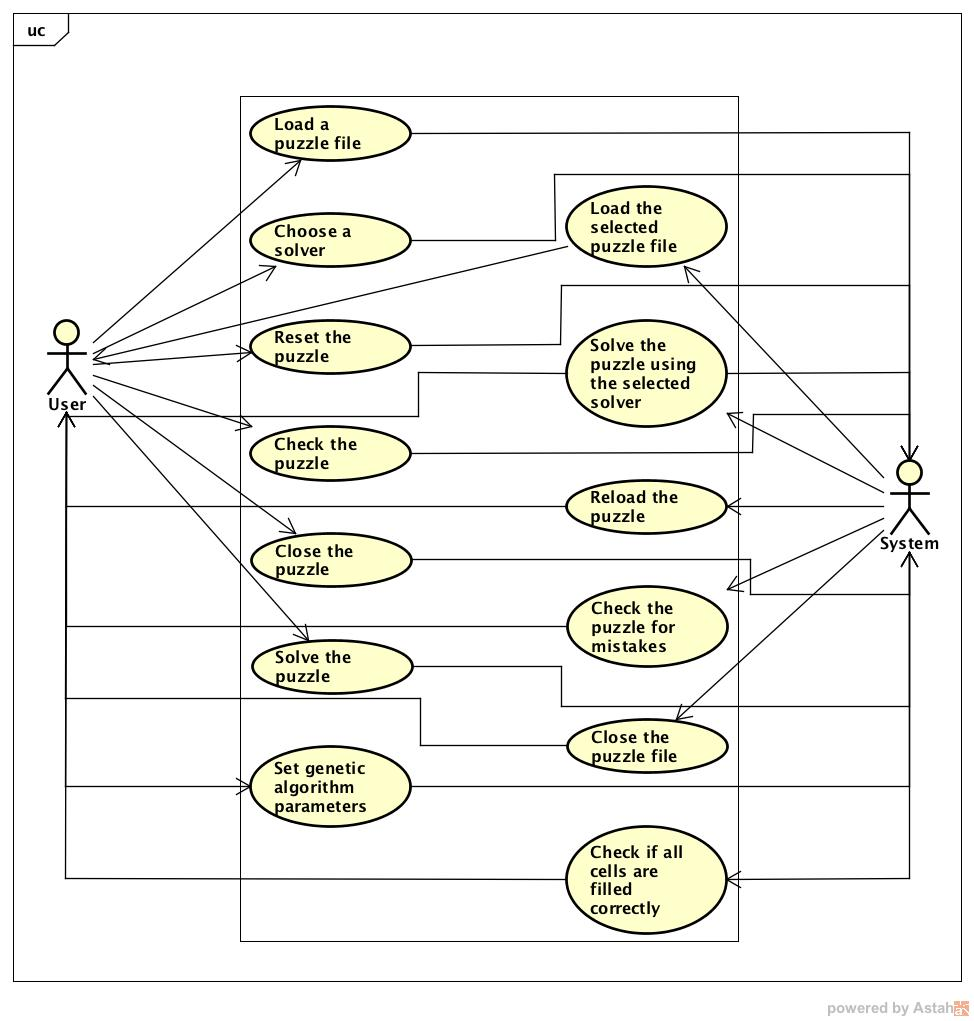
\includegraphics[scale=0.2]{Gambar/Analisis/DiagramUseCase}
\caption[Diagram \textit{use case} untuk perangkat lunak permainan teka-teki Calcudoku]{Diagram \textit{use case} untuk perangkat lunak permainan teka-teki Calcudoku}
\label{fig:analisisusecase}
\end{figure}
\end{frame}

\note{

}

\section{Perancangan}

\begin{frame}
\frametitle{Perancangan Masukan}
\begin{itemize}
\item Masukan untuk perangkat lunak Calcudoku ini berupa sebuah \textit{file} teks, seperti yang ditunjukkan pada Gambar~\ref{fig:perancanganmasukan}.
\end{itemize}
\begin{figure}
\centering
\captionsetup{justification=centering}
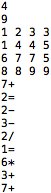
\includegraphics[scale=0.75]{Gambar/Perancangan/PerancanganInput.png}
\caption[Contoh \textit{file} masukan.]{Contoh \textit{file} masukan.}
\label{fig:perancanganmasukan}
\end{figure}
\end{frame}

\note{
Masukan untuk perangkat lunak permainan teka-teki Calcudoku ini berupa sebuah \textit{file} teks, seperti yang ditunjukkan pada Gambar~\ref{fig:perancanganmasukan}.
}

\begin{frame}
\frametitle{Perancangan Masukan}
\begin{itemize}
\item Adapun rincian dari \textit{file} teks masukan tersebut adalah sebagai berikut:
	\begin{enumerate}
	\item Baris pertama berisi ukuran \textit{grid} dan banyaknya \textit{cage} dari teka-teki Calcudoku tersebut.
	\item Baris kedua sampai ke baris ke-\begin{math}2 + (n - 1)\end{math}, dengan \begin{math}n\end{math} adalah ukuran \textit{grid}, berisi matriks \textit{cage assignment}.
	\item Baris ke-\begin{math}2 + n\end{math} dan seterusnya berisi \textit{cage objectives} untuk setiap \textit{cage}.
	\end{enumerate}
\end{itemize}
\end{frame}

\note{
Adapun rincian dari \textit{file} teks masukan tersebut adalah sebagai berikut:
\begin{enumerate}
\item Baris pertama berisi ukuran \textit{grid} dan banyaknya \textit{cage} dari teka-teki Calcudoku tersebut. Angka pertama adalah ukuran \textit{grid}, dan angka kedua adalah banyaknya \textit{cage}.
\item Baris kedua sampai ke baris ke-\begin{math}2 + (n - 1)\end{math}, dengan \begin{math}n\end{math} adalah ukuran \textit{grid}, berisi matriks \textit{cage assignment}. Matriks ini merepresentasikan posisi dari setiap \textit{cage} dalam \textit{grid}. Setiap \textit{cage} direpresentasikan dengan angka yang berbeda. Setiap \textit{cage} dapat mempunyai ukuran (jumlah sel yang terdapat dalam \textit{cage}) yang bervariasi. Setiap sel dalam sebuah \textit{cage} harus berhubungan secara horizontal atau vertikal dengan sel lain dalam \textit{cage} yang sama.
\item Baris ke-\begin{math}2 + n\end{math} dan seterusnya berisi \textit{cage objectives} untuk setiap \textit{cage}. \textit{Cage objectives} berisikan angka tujuan dan operasi matematika yang telah ditentukan. Angka-angka dalam sebuah \textit{cage} harus mencapai angka tujuan jika dihitung menggunakan operasi matematika yang telah ditentukan.
\end{enumerate}
}

\begin{frame}
\frametitle{Perancangan Keluaran}
\begin{itemize}
\item Keluaran untuk perangkat lunak Calcudoku ini berupa sebuah matriks yang berisi solusi dari teka-teki Calcudoku yang sudah diselesaikan oleh program, seperti dapat dilihat pada Gambar~\ref{fig:perancangankeluaran}.
\end{itemize}
\begin{figure}
\centering
\captionsetup{justification=centering}
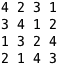
\includegraphics[scale=1]{Gambar/Perancangan/PerancanganOutput.png}
\caption[Contoh keluaran.]{Contoh keluaran.}
\label{fig:perancangankeluaran}
\end{figure}
\end{frame}

\note{
Keluaran untuk perangkat lunak permainan teka-teki Calcudoku ini berupa sebuah matriks yang berisi solusi dari teka-teki Calcudoku yang sudah diselesaikan oleh program, seperti dapat dilihat pada Gambar~\ref{fig:perancangankeluaran}.
}

\begin{frame}
\frametitle{Perancangan Antarmuka}
\begin{itemize}
\item Antarmuka ini terdiri dari sebuah \textit{frame} yang berisi sebuah menu \textit{bar} dan GUI dari  Calcudoku.
\item GUI hanya akan ditampilkan jika sudah membuka \textit{file} permainan. Jika \textit{file} permainan ditutup, maka GUI juga akan ditutup.
\item Menu \textit{bar} terdiri dari dua menu, yaitu:
	\begin{enumerate}
	\item \textit{File}
	\item \textit{Solve}
	\end{enumerate}
\end{itemize}
\end{frame}

\note{
Antarmuka untuk perangkat lunak ini terdiri dari sebuah \textit{frame} yang berisi sebuah menu \textit{bar} dan GUI dari permainan teka-teki Calcudoku. GUI hanya akan ditampilkan jika perangkat lunak sudah membuka \textit{file} permainan. Jika \textit{file} permainan ditutup, maka GUI juga akan ditutup.

Menu \textit{bar} untuk perangkat lunak ini terdiri dari dua menu, yaitu:
\begin{enumerate}
\item \textit{File}, yaitu menu yang berisi \textit{item-item} menu yang terkait dengan \textit{file} permainan.
\item \textit{Solve}, yaitu menu yang berisi \textit{item-item} menu yang terkait dengan \textit{solver}.
\end{enumerate}
}

\begin{frame}
\frametitle{Perancangan Antarmuka}
\begin{itemize}
\item Gambar~\ref{fig:perancangangui1} menunjukkan perancangan GUI sebelum \textit{file} permainan dibuka. 
\end{itemize}
\begin{figure}
\centering
\captionsetup{justification=centering}

\includegraphics[scale=0.4]{Gambar/Perancangan/PerancanganGUI1.png}
\caption[Perancangan GUI sebelum \textit{file} permainan dibuka.]{Perancangan GUI sebelum membuka \textit{file} permainan}
\label{fig:perancangangui1}
\end{figure}
\end{frame}

\note{
Gambar~\ref{fig:perancangangui1} menunjukkan perancangan GUI sebelum \textit{file} permainan dibuka. 
}

\begin{frame}
\frametitle{Perancangan Antarmuka}
\begin{itemize}
\item Gambar~\ref{fig:perancangangui2} menunjukkan perancangan GUI sesudah \textit{file} permainan dibuka. 
\end{itemize}
\begin{figure}
\centering
\captionsetup{justification=centering}
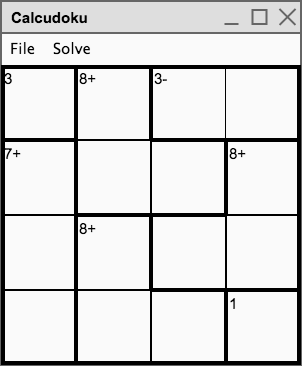
\includegraphics[scale=0.4]{Gambar/Perancangan/PerancanganGUI2.png}
\caption[Perancangan GUI sesudah \textit{file} permainan dibuka.]{Perancangan GUI sesudah membuka \textit{file} permainan}
\label{fig:perancangangui2}
\end{figure}
\end{frame}

\note{
Gambar~\ref{fig:perancangangui2} menunjukkan perancangan GUI sesudah \textit{file} permainan dibuka. 
}

\begin{frame}
\frametitle{Perancangan Antarmuka}
\begin{itemize}
\item Gambar~\ref{fig:perancangangui3} menunjukkan perancangan GUI sesudah permainan berdasarkan \textit{file} permainan yang dibuka diselesaikan.
\end{itemize}
\begin{figure}
\centering
\captionsetup{justification=centering}
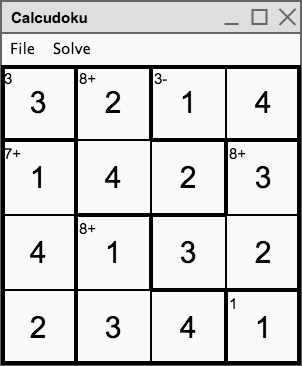
\includegraphics[scale=0.4]{Gambar/Perancangan/PerancanganGUI3.png}
\caption[Perancangan GUI sesudah permainan berdasarkan \textit{file} permainan yang dibuka diselesaikan.]{Perancangan GUI sesudah permainan berdasarkan \textit{file} permainan yang dibuka diselesaikan.}
\label{fig:perancangangui3}
\end{figure}
\end{frame}

\note{
Gambar~\ref{fig:perancangangui3} menunjukkan perancangan GUI sesudah permainan berdasarkan \textit{file} permainan yang dibuka diselesaikan.
}

\begin{frame}
\frametitle{Perancangan Antarmuka - Menu \textit{File}}
\begin{itemize}
\item Menu \textit{File} mempunyai beberapa menu \textit{item}, yaitu:
	\begin{enumerate}
	\item \textit{Load Puzzle File}
	\item \textit{Reset Puzzle}
	\item \textit{Close Puzzle File}
	\item \textit{Check Puzzle}
	\item \textit{Exit}
	\end{enumerate}
\item Gambar~\ref{fig:perancanganguimenufile} menunjukkan isi dari menu \textit{File}.
\end{itemize}
\begin{figure}
\centering
\captionsetup{justification=centering}
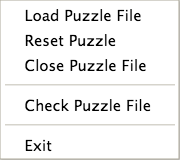
\includegraphics[scale=0.5]{Gambar/Perancangan/PerancanganGUIMenuFile.png}
\caption[Menu \textit{File}]{Menu \textit{File}}
\label{fig:perancanganguimenufile}
\end{figure}
\end{frame}

\note{
Menu \textit{File} mempunyai beberapa menu \textit{item}, yaitu:
\begin{enumerate}
\item \textit{Load Puzzle File}, yaitu menu \textit{item} untuk membuka \textit{file} permainan.
\item \textit{Reset Puzzle}, yaitu menu \textit{item} untuk me-\textit{reset} permainan.
\item \textit{Close Puzzle File}, yaitu menu \textit{item} untuk menutup \textit{file} permainan.
\item \textit{Check Puzzle}, yaitu menu \textit{item} untuk memeriksa permainan jika ada masukan yang salah di dalam \textit{grid}.
\item \textit{Exit}, yaitu menu \textit{item} untuk menutup perangkat lunak.
\end{enumerate}
Gambar~\ref{fig:perancanganguimenufile} menunjukkan isi dari menu \textit{File}.
}

\begin{frame}
\frametitle{Perancangan Antarmuka - Menu \textit{Solve}}
\begin{itemize}
\item Menu \textit{Solve} mempunyai beberapa menu \textit{item}, yaitu:
	\begin{enumerate}
	\item \textit{Backtracking}
	\item \textit{Hybrid Genetic}
	\item \textit{Set Genetic Algorithm Parameters}
	\end{enumerate}
\item Gambar~\ref{fig:perancanganguimenusolve} menunjukkan isi dari menu \textit{Solve}.
\end{itemize}
\begin{figure}
\centering
\captionsetup{justification=centering}
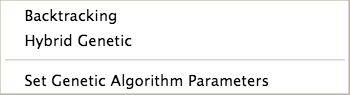
\includegraphics[scale=0.5]{Gambar/Perancangan/PerancanganGUIMenuSolve.png}
\caption[Menu \textit{Solve}]{Menu \textit{Solve}}
\label{fig:perancanganguimenusolve}
\end{figure}
\end{frame}

\note{
Menu \textit{Solve} mempunyai beberapa menu \textit{item}, yaitu:
\begin{enumerate}
\item \textit{Backtracking}, yaitu menu \textit{item} untuk menyelesaikan permainan berdasarkan \textit{file} permainan yang dibuka dengan algoritma \textit{backtracking}.
\item \textit{Hybrid Genetic}, yaitu menu \textit{item} untuk menyelesaikan permainan berdasarkan \textit{file} permainan yang dibuka dengan algoritma \textit{hybrid genetic}.
\item \textit{Set Genetic Algorithm Parameters}, yaitu menu \textit{item} untuk mengatur nilai dari parameter-parameter untuk algoritma genetik.
\end{enumerate}
Gambar~\ref{fig:perancanganguimenusolve} menunjukkan isi dari menu \textit{Solve}.
}

\begin{frame}
\frametitle{Diagram Kelas}
\begin{itemize}
\item Perangkat lunak Calcudoku ini terdiri dari beberapa kelas, yang dikelompokkan dalam tiga package, yaitu:
	\begin{enumerate}
	\item Model
	\item View
	\item Controller
	\end{enumerate}
\item Diagram kelas untuk perangkat lunak ini dapat dilihat pada Gambar~\ref{fig:diagramkelas}.
\end{itemize}
\end{frame}

\note{
Perangkat lunak teka-teki Calcudoku ini terdiri dari beberapa kelas, yang dikelompokkan dalam tiga package, yaitu:
\begin{enumerate}
\item Model, yaitu \textit{engine} dari perangkat lunak ini.
\item View, yaitu GUI dari perangkat lunak ini.
\item Controller, yaitu penghubung antara \textit{package} model dan \textit{package} view
\end{enumerate}
Diagram kelas untuk perangkat lunak ini dapat dilihat pada Gambar~\ref{fig:diagramkelas}.
}

\begin{frame}
\frametitle{Diagram Kelas}
\begin{figure}
\centering
\captionsetup{justification=centering}
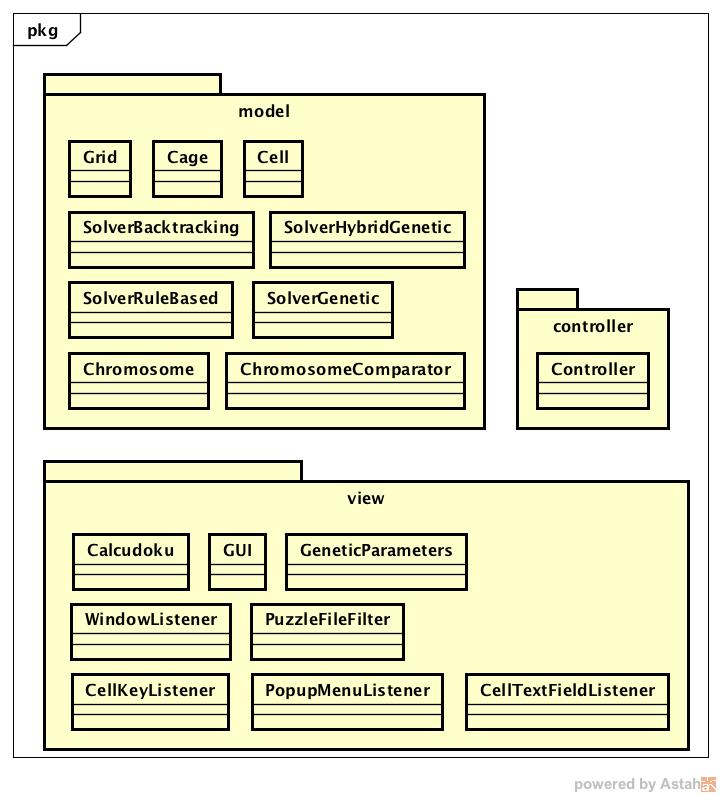
\includegraphics[scale=0.25]{Gambar/Perancangan/DiagramKelas.jpg}
\caption[Diagram kelas untuk perangkat lunak Calcudoku.]{Diagram kelas untuk perangkat lunak Calcudoku.}
\label{fig:diagramkelas}
\end{figure}
\end{frame}

\note{

}

\begin{frame}
\frametitle{Diagram Kelas - \textit{Package} Model}
\begin{itemize}
\item \textit{Package} model memiliki beberapa kelas, yaitu:
	\begin{enumerate}
	\item Grid
	\item Cell
	\item Cage
	\item SolverBacktracking
	\item SolverHybridGenetic
	\item SolverRuleBased
	\end{enumerate}
\end{itemize}
\end{frame}

\note{
\textit{Package} model memiliki beberapa kelas, yaitu:
\begin{enumerate}
\item Grid, yaitu kelas yang merepresentasikan \textit{grid} dalam teka-teki Calcudoku.
\item Cell, yaitu kelas yang merepresentasikan sel dalam teka-teki Calcudoku.
\item Cage, yaitu kelas yang merepresentasikan \textit{cage} dalam teka-teki Calcudoku.
\item SolverBacktracking, yaitu kelas \textit{solver} untuk teka-teki Calcudoku menggunakan algoritma backtracking.
\item SolverHybridGenetic, yaitu kelas \textit{solver} untuk teka-teki Calcudoku menggunakan algoritma \textit{hybrid genetic}. Algoritma ini akan mencoba menyelesaikan teka-teki Calcudoku menggunakan algoritma \textit{rule based} terlebih dahulu. Algoritma genetik baru akan dijalankan jika algoritma \textit{rule based} gagal dalam menyelesaikan teka-teki Calcudoku.
\item SolverRuleBased, yaitu kelas \textit{solver} untuk teka-teki Calcudoku menggunakan algoritma \textit{rule based}. Dalam algoritma \textit{hybrid genetic}, algoritma akan mencoba menyelesaikan teka-teki Calcudoku menggunakan algoritma \textit{rule based} terlebih dahulu.
\end{enumerate}
}

\begin{frame}
\frametitle{Diagram Kelas - \textit{Package} Model dan Controller}
\begin{itemize}
\item \textit{Package} model memiliki beberapa kelas, yaitu:
	\begin{enumerate} \addtocounter{enumi}{6}
	\item SolverGenetic
	\item Chromosome
	\item ChromosomeComparator
	\end{enumerate}
\item \textit{Package} controller hanya memiliki satu kelas, yaitu kelas Controller.
\end{itemize}
\end{frame}

\note{
\textit{Package} model memiliki beberapa kelas, yaitu:
\begin{enumerate} \addtocounter{enumi}{6}
\item SolverGenetic, yaitu kelas \textit{solver} untuk teka-teki Calcudoku menggunakan algoritma genetik. Dalam algoritma \textit{hybrid genetic}, algoritma genetik baru akan dijalankan jika algoritma \textit{rule based} gagal dalam menyelesaikan teka-teki Calcudoku.
\item Chromosome, yaitu kelas yang merepresentasikan sebuah kromosom untuk algoritma genetik dalam solver \textit{hybrid genetic}.
\item ChromosomeComparator, yaitu kelas pembanding \textit{custom} (\textit{custom comparator}) yang berfungsi untuk mengurutkan kromosom berdasarkan nilai kelayakkannya (\textit{fitness value}).
\end{enumerate}
\textit{Package} model memiliki satu kelas, yaitu kelas Controller. Kelas ini berfungsi untuk menghubungkan kelas-kelas dalam \textit{package} model dengan kelas-kelas dalam \textit{package} view.
}

\begin{frame}
\frametitle{Diagram Kelas - \textit{Package} View}
\begin{itemize}
\item \textit{Package} view memiliki beberapa kelas, yaitu:
	\begin{enumerate}
	\item Calcudoku
	\item PuzzleFileFilter
	\item GUI
	\item CellKeyListener
	\item PopupMenuListener
	\item CellTextFieldListener
	\item GeneticParameters
	\end{enumerate}
\end{itemize}
\end{frame}

\note{
\textit{Package} view memiliki beberapa kelas, yaitu:
\begin{enumerate}
\item Calcudoku, yaitu kelas \textit{frame} yang berisi menu \textit{bar} dan instansiasi kelas panel GUI.
\item WindowListener, yaitu kelas \textit{listener} untuk kelas Calcudoku. \textit{Listener} ini berfungsi untuk menambahkan pesan peringatan saat akan menutup perangkat lunak.
\item PuzzleFileFilter, yaitu kelas filter untuk \textit{file chooser}. Filter ini membatasi agar \textit{file chooser} hanya bisa membuka \textit{file} teks.
\item GUI, yaitu kelas panel yang merepresentasikan GUI dari permainan teka-teki Calcudoku.
\item CellKeyListener, yaitu kelas \textit{listener} untuk kelas GUI. \textit{Listener} ini berfungsi untuk menggerakkan kursor dari sebuah sel ke sel di sebelahnya menggunakan tombol-tombol panah ke kiri, ke atas, ke bawah, dan ke kanan. Listener ini juga berfungsi untuk membatasi agar sel hanya bisa diisi oleh satu angka.
\item PopupMenuListener, yaitu kelas \textit{listener} untuk kelas GUI. \textit{Listener} ini berfungsi untuk mengisi sel dengan angka menggunakan menu \textit{pop up}, sel akan diisi dengan angka yang dipilih.
\item CellTextFieldListener, yaitu kelas \textit{listener} untuk kelas GUI. \textit{Listener} ini berfungsi untuk mengisikan sel dalam kelas Grid dengan angka yang diisikan ke dalam sel dalam GUI.
\item GeneticParameters, yaitu kelas yang berisi \textit{form} untuk mengatur nilai dari parameter-parameter untuk algoritma genetik.
\end{enumerate}
}

\section{Kode Program}

\begin{frame}[fragile]
\frametitle{Kode Program - Algoritma \textit{Backtracking}}
\begin{itemize}
\item Isilah mulai dari sel pada sudut kiri atas.
\item Algoritma \textit{backtracking} selesai jika semua sel sudah terisi dengan benar.
\end{itemize}
\begin{lstlisting}[basicstyle=\tiny]
    public boolean solve()
    {
        if (solve(0, 0) == true)
        {
            this.solution = grid;
            ...
            return true;
        }
        else
        {
            return false;
        }
    }
\end{lstlisting}
\end{frame}

\note{
Isilah mulai dari sel pada sudut kiri atas. Algoritma selesai jika semua sel sudah terisi dengan benar.
}

\begin{frame}[fragile]
\frametitle{Kode Program - Algoritma \textit{Backtracking}}
\begin{itemize}
\item Jika sudah mengisi sel yang paling kanan, isilah sel yang paling kiri pada baris berikutnya.
\end{itemize}
\begin{lstlisting}[basicstyle=\tiny]
    private boolean solve(int row, int column)
    {
        if (column >= size)
        {
            column = 0;
            row++;
            if (row >= size)
            {
                ...
                return true;
            }
        }
        ...
\end{lstlisting}
\end{frame}

\note{
Jika sudah mengisi sel yang paling kanan, isilah sel paling kiri pada baris berikutnya.
}

\begin{frame}[fragile]
\frametitle{Kode Program - Algoritma \textit{Backtracking}}
\begin{itemize}
\item Setelah mengisi sebuah sel, isilah sel di sebelah kanannya.
\item Jika semua kemungkinan gagal, mundur ke tahap sebelumnya, dan cobalah kemungkinan berikutnya.
\end{itemize}
\begin{lstlisting}[basicstyle=\tiny]
        ...
        for (int value = 1; value <= size; value++)
        {
            ...
            if (grid.solverSetCellValue(row, column, value))
            {
                if (solve(row, column + 1))
                {
                    return true;
                }
            }
        }
        ...
        grid.unsetCellValue(row, column);
        return false;
    }
\end{lstlisting}
\end{frame}

\note{
Setelah mengisi sebuah sel, isilah sel di sebelah kanannya. Jika semua kemungkinan gagal, mundur ke tahap sebelumnya, dan cobalah kemungkinan berikutnya
}

\begin{frame}[fragile]
\frametitle{Kode Program - Algoritma \textit{Hybrid Genetic}}
\begin{itemize}
\item \textit{Solver} akan mencoba menyelesaikan permainan dengan algoritma \textit{rule based}.
\end{itemize}
\begin{lstlisting}[basicstyle=\tiny]
    public boolean solve()
    {
        SolverRuleBased srb = new SolverRuleBased(grid);
        boolean isFilled = srb.solve();
        this.gridRuleBased = srb.getGrid();
        if (isFilled)
        {
            this.solution = srb.getSolution();
            ...
            return true;
        }
        ...
\end{lstlisting}
\end{frame}

\note{
\textit{Solver} akan mencoba menyelesaikan permainan dengan algoritma \textit{rule based}.
}

\begin{frame}[fragile]
\frametitle{Kode Program - Algoritma \textit{Hybrid Genetic}}
\begin{itemize}
\item Jika algoritma \textit{rule based} tidak berhasil mengisi semua sel dalam \textit{grid} dengan benar, maka \textit{solver} akan mencoba menyelesaikan permainan dengan algoritma genetik.
\end{itemize}
\begin{lstlisting}[basicstyle=\tiny]
	...
        else
        {
            SolverGenetic sg = new SolverGenetic(gridRuleBased, 
                    generations, populationSize, elitismRate, 
                    crossoverRate, mutationRate);
            if (sg.solve() == true)
            {
                this.solution = sg.getSolution();
                ...
                return true;
            }
        }
        return false;
    }
\end{lstlisting}
\end{frame}

\note{
Jika algoritma \textit{rule based} tidak berhasil mengisi semua sel dalam \textit{grid} dengan benar, maka \textit{solver} akan mencoba menyelesaikan permainan dengan algoritma genetik.
}

\begin{frame}[fragile]
\frametitle{Kode Program - Algoritma \textit{Rule Based}}
\begin{itemize}
\item Algoritma \textit{rule based} dimulai dengan mengaplikasikan aturan logika \textit{single square} dan aturan logika \textit{killer combination}.
\item Kedua aturan logika ini hanya diaplikasikan sekali, yaitu di awal algoritma.
\end{itemize}
\begin{lstlisting}[basicstyle=\tiny]
    public boolean solve()
    {
        singleSquare();
        killerCombination();;
        ...
\end{lstlisting}
\end{frame}

\note{
Algoritma \textit{rule based} dimulai dengan mengaplikasikan aturan logika \textit{single square} dan aturan logika \textit{killer combination}. Kedua aturan logika ini hanya diaplikasikan sekali, yaitu di awal algoritma.
}

\begin{frame}[fragile]
\frametitle{Kode Program - Algoritma \textit{Rule Based}}
\begin{itemize}
\item Algoritma lalu mengaplikasikan aturan logika \textit{naked subset} dan aturan logika \textit{hidden single}.
\item Kedua aturan logika ini diulang sampai algoritma tidak bisa lagi mengisi sel-sel dalam \textit{grid} atau sampai semua sel dalam \textit{grid} sudah terisi dengan benar.
\end{itemize}
\begin{lstlisting}[basicstyle=\tiny]
	...
        ArrayList<ArrayList<Integer>> currentGridArrayList 
                = getGridArrayList();
        ArrayList<ArrayList<Integer>> newGridArrayList 
                = solveLoop();
        while(!currentGridArrayList.equals(newGridArrayList))
        {
            ...
            currentGridArrayList = newGridArrayList;
            newGridArrayList = solveLoop();
        }
	...
\end{lstlisting}
\end{frame}

\note{
Algoritma lalu mengaplikasikan aturan logika \textit{naked subset} dan aturan logika \textit{hidden single}.
Kedua aturan logika ini diulang sampai algoritma tidak bisa lagi mengisi sel-sel dalam \textit{grid} atau sampai semua sel dalam \textit{grid} sudah terisi dengan benar.
}

\begin{frame}[fragile]
\frametitle{Kode Program - Algoritma \textit{Rule Based}}
\begin{itemize}
\item Algoritma \textit{hybrid genetic} selesai jika semua sel dalam \textit{grid} sudah terisi dengan benar.
\item Algoritma genetik akan dimulai jika ada sel-sel di dalam \textit{grid} yang masih kosong.
\end{itemize}
\begin{lstlisting}[basicstyle=\tiny]
	...
        if (grid.isFilled())
        {
            this.solution = grid;
            return true;
        }
        else
        {
            return false;
        }
    }
\end{lstlisting}
\end{frame}

\note{
Algoritma \textit{hybrid genetic} selesai jika semua sel dalam \textit{grid} sudah terisi dengan benar. Algoritma genetik akan dimulai jika ada sel-sel di dalam \textit{grid} yang masih kosong.
}

\begin{frame}[fragile]
\frametitle{Kode Program - Algoritma Genetik}
\begin{itemize}
\item Algoritma genetik dimulai dengan membangkitkan generasi awal secara acak.
\end{itemize}
\begin{lstlisting}[basicstyle=\tiny]
    public SolverGenetic(...)
    {
        ...
        generatePopulation();
	...
    }
\end{lstlisting}
\end{frame}

\note{
Algoritma genetik dimulai dengan membangkitkan generasi awal secara acak.
}

\begin{frame}[fragile]
\frametitle{Kode Program - Algoritma Genetik}
\begin{itemize}
\item Setiap kromosom dalam sebuah generasi dihitung nilai kelayakannya.
\item Nilai kelayakan untuk sebuah kromosom adalah jumlah sel yang sudah diisi dengan benar dibagi dengan jumlah semua sel yang ada di dalam \textit{grid}.
\end{itemize}
\begin{lstlisting}[basicstyle=\tiny]
    private double setFitness()
    {
        double numberOfValidCells = 0;
        double numberOfCells = size * size;
        for (int i = 0; i < size; i++)
        {
            for (int j = 0; j < size; j++)
            {
                if (grid.solverIsCellValueValid(i, j) == true)
                {
                    numberOfValidCells++;
                }
            }
        }
        double value = numberOfValidCells / numberOfCells;
        return value;
    }
\end{lstlisting}
\end{frame}

\note{
Setiap kromosom dalam sebuah generasi dihitung nilai kelayakannya. Nilai kelayakan untuk sebuah kromosom adalah jumlah sel yang sudah diisi dengan benar dibagi dengan jumlah semua sel yang ada di dalam \textit{grid}.
}

\begin{frame}[fragile]
\frametitle{Kode Program - Algoritma Genetik}
\begin{itemize}
\item Algoritma selesai jika solusi ditemukan.
\item Solusi adalah kromosom dengan nilai kelayakan 1.
\end{itemize}
\begin{lstlisting}[basicstyle=\tiny]
    public boolean solve()
    {
        for (int i = 0; i < generations; i++)
        {
            solveLoop();
            sortChromosomes();
            for (int j = 0; j < populationSize; j++)
            {
                ...
                if (currentGeneration.get(j).getFitness() == 1.0)
                {
                    this.solution 
                            = currentGeneration.get(j).getGrid();
                    return true;
                }
            }
        }
        return false;
    }
\end{lstlisting}
\end{frame}

\note{
Algoritma selesai jika solusi ditemukan. Solusi adalah kromosom dengan nilai kelayakan 1.
}

\begin{frame}[fragile]
\frametitle{Kode Program - Algoritma Genetik}
\begin{itemize}
\item Jika solusi tidak ditemukan, maka algoritma genetik akan membangkitkan generasi berikutnya, sampai solusi ditemukan.
\end{itemize}
\begin{lstlisting}[basicstyle=\tiny]
    private void solveLoop()
    {      
        int elitismNumber 
                = (int) Math.round(populationSize * elitismRate);
        int mutationNumber
                = (int) Math.round(populationSize * mutationRate);
        int crossoverNumber
                =  (int) Math.round((populationSize * crossoverRate)
                        / 2);
        sortChromosomes();
        ...
\end{lstlisting}
\end{frame}

\note{
Jika solusi tidak ditemukan, maka algoritma genetik akan membangkitkan generasi berikutnya, sampai solusi ditemukan.
}

\begin{frame}[fragile]
\frametitle{Kode Program - Algoritma Genetik}
\begin{itemize}
\item Generasi berikutnya dibangkitkan dari generasi sebelumnya menggunakan operator-operator algoritma genetik, seperti \textit{elitism}, kawin silang, dan mutasi.
\end{itemize}
\begin{lstlisting}[basicstyle=\tiny]
	...
        for (int i = 0; i < elitismNumber; i++)
        {
            if (!nextGeneration.contains(currentGeneration.get(i)))
            {
                nextGeneration.add(cloneChromosome(
                        currentGeneration.get(i)));
            }
        }
        for (int i = 0; i < mutationNumber; i++)
        {
            Chromosome parent = randomSelection(currentGeneration);
            nextGeneration.add(mutation(parent));
        }
        for (int i = 0; i < crossoverNumber; i++)
        {
            nextGeneration.addAll(crossover(
                    randomSelection(currentGeneration),
                    randomSelection(currentGeneration)));
        }
        ...
        currentGeneration = nextGeneration;
        nextGeneration = new ArrayList<Chromosome>();
    }
\end{lstlisting}
\end{frame}

\note{
Generasi berikutnya dibangkitkan dari generasi sebelumnya menggunakan operator-operator algoritma genetik, seperti \textit{elitism}, kawin silang, dan mutasi.
}

\section{Implementasi dan Pengujian}

\begin{frame}
\frametitle{Hasil Pengujian - Algoritma \textit{Backtracking}}
\begin{itemize}
\item Pengujian algoritma \textit{backtracking} dilakukan pada permainan dengan \textit{grid} yang berukuran \begin{math}4 \times 4\end{math} sampai dengan \begin{math}8 \times 8\end{math}.
\item Hasil pengujian algoritma \textit{backtracking} dapat dilihat pada Tabel~\ref{tab:pengujianbt}.
\end{itemize}
\begin{table}
\tiny
\centering
\captionsetup{justification=centering}
\caption[Hasil pengujian algoritma \textit{backtracking} untuk Calcudoku]{Hasil pengujian algoritma \textit{backtracking} untuk Calcudoku}
\begin{tabular}{| l | l | l |}
\hline
Ukuran \textit{Grid} & \makecell[c]{Rata-Rata \\ Tingkat Keberhasilan} & \makecell[c]{Rata-Rata \\ Kecepatan} \\
\hline \hline
\begin{math}4 \times 4\end{math} & 100\% & 0.067 detik \\
\hline
\begin{math}5 \times 5\end{math} & 100\% & 0.701 detik \\
\hline
\begin{math}6 \times 6\end{math} & 100\% & 13.84 detik \\
\hline
\begin{math}7 \times 7\end{math} & 100\% & 482.653 detik \\
\hline
\begin{math}8 \times 8\end{math} & 100\% & 2134.655 detik \\
\hline
\end{tabular}
\label{tab:pengujianbt}
\end{table}
\end{frame}

\note{
Pengujian algoritma \textit{backtracking} dilakukan pada permainan degan \textit{grid} berukuran \begin{math}4 \times 4\end{math} sampai dengan \begin{math}8 \times 8\end{math}. Hasil pengujian algoritma \textit{backtracking} dapat dilihat pada Tabel~\ref{tab:pengujianbt}.
}

\begin{frame}
\frametitle{Hasil Pengujian - Algoritma \textit{Hybrid Genetic}}
\begin{itemize}
\item Pengujian algoritma \textit{hybrid genetic} dilakukan pada \textit{grid} dengan ukuran \begin{math}4 \times 4\end{math} sampai dengan \begin{math}8 \times 8\end{math}.
\item Dilakukan 16 skenario pengujian.
\item Nilai dari parameter-parameter untuk algoritma genetik berbeda-beda untuk setiap skenario.
\item Daftar nilai dari parameter-parameter untuk algoritma genetik untuk setiap skenario dapat dilihat pada Tabel~\ref{tab:nilaiparameterhg}.
\end{itemize}
\end{frame}

\note{
Pengujian algoritma \textit{hybrid genetic} dilakukan pada \textit{grid} dengan ukuran \begin{math}4 \times 4\end{math} sampai dengan \begin{math}8 \times 8\end{math}. Dilakukan 16 skenario pengujian. Nilai dari parameter-parameter untuk algoritma genetik berbeda-beda untuk setiap skenario. Daftar nilai dari parameter-parameter untuk algoritma genetik untuk setiap skenario dapat dilihat pada Tabel~\ref{tab:nilaiparameterhg}.
}

\begin{frame}
\frametitle{Hasil Pengujian - Algoritma \textit{Hybrid Genetic}}
\begin{table}
\tiny
\centering
\captionsetup{justification=centering}
\caption[Nilai untuk parameter-parameter algoritma genetik untuk setiap percobaan yang dilakukan]{Nilai untuk parameter-parameter algoritma genetik untuk setiap percobaan yang dilakukan}
\begin{tabular}{| l | l | l | l | l | l |}
\hline
Skenario & Populasi & Generasi & \textit{Elitism} & Mutasi & Kawin Silang \\
\hline \hline
1 & 1000 & 100 & 10\% & 10\% & 80\% \\
\hline
2 & 1000 & 100 & 5\% & 10\% & 85\% \\
\hline
3 & 1000 & 100 & 10\% & 5\% & 85\% \\
\hline
4 & 1000 & 100 & 5\% & 5\% & 90\% \\
\hline
5 & 100 & 100 & 10\% & 10\% & 80\% \\
\hline
6 & 100 & 100 & 5\% & 10\% & 85\% \\
\hline
7 & 100 & 100 & 10\% & 5\% & 85\% \\
\hline
8 & 100 & 100 & 5\% & 5\% & 90\% \\
\hline
9 & 1000 & 10 & 10\% & 10\% & 80\% \\
\hline
10 & 1000 & 10 & 5\% & 10\% & 85\% \\
\hline
11 & 1000 & 10 & 10\% & 5\% & 85\% \\
\hline
12 & 1000 & 10 & 5\% & 5\% & 90\% \\
\hline
13 & 100 & 10 & 10\% & 10\% & 80\% \\
\hline
14 & 100 & 10 & 5\% & 10\% & 85\% \\
\hline
15 & 100 & 10 & 10\% & 5\% & 85\% \\
\hline
16 & 100 & 10 & 5\% & 5\% & 90\% \\
\hline
\end{tabular}
\label{tab:nilaiparameterhg}
\end{table}

\end{frame}

\note{

}

\begin{frame}
\frametitle{Hasil Pengujian - Algoritma \textit{Hybrid Genetic}}
\begin{itemize}
\item Hasil pengujian algoritma \textit{hybrid genetic} untuk Skenario 1 dapat dilihat pada Tabel~\ref{tab:pengujianhg1}.
\end{itemize}
\begin{table}
\tiny
\centering
\captionsetup{justification=centering}
\caption[Hasil pengujian algoritma \textit{hybrid genetic} untuk Calcudoku (Skenario 1)]{Hasil pengujian algoritma \textit{hybrid genetic} untuk Calcudoku (Skenario 1)}
\begin{tabular}{| l | l | l | l |}
\hline
Ukuran \textit{Grid} & \makecell[c]{Rata-Rata \\ Tingkat Keberhasilan} & \makecell[c]{Rata-Rata \\ Kecepatan} & \makecell[c]{Rata-Rata Jumlah Sel \\ Diisi Algoritma \textit{Rule Based}} \\
\hline \hline
\begin{math}4 \times 4\end{math} & 100\% & 3.735 detik & 3 \\
\hline
\begin{math}5 \times 5\end{math} & 42.308\% & 8.389 detik & 9 \\
\hline
\begin{math}6 \times 6\end{math} & 0\% & - & - \\
\hline
\begin{math}7 \times 7\end{math} & 0\% & - & - \\
\hline
\begin{math}8 \times 8\end{math} & 0\% & - & - \\
\hline
\end{tabular}
\label{tab:pengujianhg1}
\end{table}
\end{frame}

\note{
Hasil pengujian algoritma \textit{hybrid genetic} untuk Skenario 1 dapat dilihat pada Tabel~\ref{tab:pengujianhg1}.
}

\begin{frame}
\frametitle{Hasil Pengujian - Algoritma \textit{Hybrid Genetic}}
\begin{itemize}
\item Hasil pengujian algoritma \textit{hybrid genetic} untuk Skenario 2 dapat dilihat pada Tabel~\ref{tab:pengujianhg2}.
\end{itemize}
\begin{table}
\tiny
\centering
\captionsetup{justification=centering}
\caption[Hasil pengujian algoritma \textit{hybrid genetic} untuk Calcudoku (Skenario 2)]{Hasil pengujian algoritma \textit{hybrid genetic} untuk Calcudoku (Skenario 2)}
\begin{tabular}{| l | l | l | l |}
\hline
Ukuran \textit{Grid} & \makecell[c]{Rata-Rata \\ Tingkat Keberhasilan} & \makecell[c]{Rata-Rata \\ Kecepatan} & \makecell[c]{Rata-Rata Jumlah Sel \\ Diisi Algoritma \textit{Rule Based}} \\
\hline \hline
\begin{math}4 \times 4\end{math} & 100\% & 4.183 detik & 3 \\
\hline
\begin{math}5 \times 5\end{math} & 42.308\% & 9.258 detik & 9 \\
\hline
\begin{math}6 \times 6\end{math} & 0\% & - & - \\
\hline
\begin{math}7 \times 7\end{math} & 0\% & - & - \\
\hline
\begin{math}8 \times 8\end{math} & 0\% & - & - \\
\hline
\end{tabular}
\label{tab:pengujianhg2}
\end{table}
\end{frame}

\note{
Hasil pengujian algoritma \textit{hybrid genetic} untuk Skenario 2 dapat dilihat pada Tabel~\ref{tab:pengujianhg2}.
}

\begin{frame}
\frametitle{Hasil Pengujian - Algoritma \textit{Hybrid Genetic}}
\begin{itemize}
\item Hasil pengujian algoritma \textit{hybrid genetic} untuk Skenario 3 dapat dilihat pada Tabel~\ref{tab:pengujianhg3}.
\end{itemize}
\begin{table}
\tiny
\centering
\captionsetup{justification=centering}
\caption[Hasil pengujian algoritma \textit{hybrid genetic} untuk Calcudoku (Skenario 3)]{Hasil pengujian algoritma \textit{hybrid genetic} untuk Calcudoku (Skenario 3)}
\begin{tabular}{| l | l | l | l |}
\hline
Ukuran \textit{Grid} & \makecell[c]{Rata-Rata \\ Tingkat Keberhasilan} & \makecell[c]{Rata-Rata \\ Kecepatan} & \makecell[c]{Rata-Rata Jumlah Sel \\ Diisi Algoritma \textit{Rule Based}} \\
\hline \hline
\begin{math}4 \times 4\end{math} & 100\% & 3.924 detik & 3 \\
\hline
\begin{math}5 \times 5\end{math} & 42.308\% & 8.806 detik & 9 \\
\hline
\begin{math}6 \times 6\end{math} & 0\% & - & - \\
\hline
\begin{math}7 \times 7\end{math} & 0\% & - & - \\
\hline
\begin{math}8 \times 8\end{math} & 0\% & - & - \\
\hline
\end{tabular}
\label{tab:pengujianhg3}
\end{table}
\end{frame}

\note{
Hasil pengujian algoritma \textit{hybrid genetic} untuk Skenario 3 dapat dilihat pada Tabel~\ref{tab:pengujianhg3}.
}

\begin{frame}
\frametitle{Hasil Pengujian - Algoritma \textit{Hybrid Genetic}}
\begin{itemize}
\item Hasil pengujian algoritma \textit{hybrid genetic} untuk Skenario 4 dapat dilihat pada Tabel~\ref{tab:pengujianhg4}.
\end{itemize}
\begin{table}
\tiny
\centering
\captionsetup{justification=centering}
\caption[Hasil pengujian algoritma \textit{hybrid genetic} untuk Calcudoku (Skenario 4)]{Hasil pengujian algoritma \textit{hybrid genetic} untuk Calcudoku (Skenario 4)}
\begin{tabular}{| l | l | l | l |}
\hline
Ukuran \textit{Grid} & \makecell[c]{Rata-Rata \\ Tingkat Keberhasilan} & \makecell[c]{Rata-Rata \\ Kecepatan} & \makecell[c]{Rata-Rata Jumlah Sel \\ Diisi Algoritma \textit{Rule Based}} \\
\hline \hline
\begin{math}4 \times 4\end{math} & 100\% & 4.371 detik & 3 \\
\hline
\begin{math}5 \times 5\end{math} & 42.308\% & 9.676 detik & 9 \\
\hline
\begin{math}6 \times 6\end{math} & 0\% & - & - \\
\hline
\begin{math}7 \times 7\end{math} & 0\% & - & - \\
\hline
\begin{math}8 \times 8\end{math} & 0\% & - & - \\
\hline
\end{tabular}
\label{tab:pengujianhg4}
\end{table}
\end{frame}

\note{
Hasil pengujian algoritma \textit{hybrid genetic} untuk Skenario 4 dapat dilihat pada Tabel~\ref{tab:pengujianhg4}.
}

\begin{frame}
\frametitle{Hasil Pengujian - Algoritma \textit{Hybrid Genetic}}
\begin{itemize}
\item Hasil pengujian algoritma \textit{hybrid genetic} untuk Skenario 5 dapat dilihat pada Tabel~\ref{tab:pengujianhg5}.
\end{itemize}
\begin{table}
\tiny
\centering
\captionsetup{justification=centering}
\caption[Hasil pengujian algoritma \textit{hybrid genetic} untuk Calcudoku (Skenario 5)]{Hasil pengujian algoritma \textit{hybrid genetic} untuk Calcudoku (Skenario 5)}
\begin{tabular}{| l | l | l | l |}
\hline
Ukuran \textit{Grid} & \makecell[c]{Rata-Rata \\ Tingkat Keberhasilan} & \makecell[c]{Rata-Rata \\ Kecepatan} & \makecell[c]{Rata-Rata Jumlah Sel \\ Diisi Algoritma \textit{Rule Based}} \\
\hline \hline
\begin{math}4 \times 4\end{math} & 56.41\% & 0.48 detik & 5 \\
\hline
\begin{math}5 \times 5\end{math} & 19.231\% & 0.311 detik & 14 \\
\hline
\begin{math}6 \times 6\end{math} & 0\% & - & - \\
\hline
\begin{math}7 \times 7\end{math} & 0\% & - & - \\
\hline
\begin{math}8 \times 8\end{math} & 0\% & - & - \\
\hline
\end{tabular}
\label{tab:pengujianhg5}
\end{table}
\end{frame}

\note{
Hasil pengujian algoritma \textit{hybrid genetic} untuk Skenario 5 dapat dilihat pada Tabel~\ref{tab:pengujianhg5}.
}

\begin{frame}
\frametitle{Hasil Pengujian - Algoritma \textit{Hybrid Genetic}}
\begin{itemize}
\item Hasil pengujian algoritma \textit{hybrid genetic} untuk Skenario 6 dapat dilihat pada Tabel~\ref{tab:pengujianhg6}.
\end{itemize}
\begin{table}
\tiny
\centering
\captionsetup{justification=centering}
\caption[Hasil pengujian algoritma \textit{hybrid genetic} untuk Calcudoku (Skenario 6)]{Hasil pengujian algoritma \textit{hybrid genetic} untuk Calcudoku (Skenario 6)}
\begin{tabular}{| l | l | l | l |}
\hline
Ukuran \textit{Grid} & \makecell[c]{Rata-Rata \\ Tingkat Keberhasilan} & \makecell[c]{Rata-Rata \\ Kecepatan} & \makecell[c]{Rata-Rata Jumlah Sel \\ Diisi Algoritma \textit{Rule Based}} \\
\hline \hline
\begin{math}4 \times 4\end{math} & 56.41\% & 0.532 detik & 5 \\
\hline
\begin{math}5 \times 5\end{math} & 19.231\% & 0.339 detik & 14 \\
\hline
\begin{math}6 \times 6\end{math} & 0\% & - & - \\
\hline
\begin{math}7 \times 7\end{math} & 0\% & - & - \\
\hline
\begin{math}8 \times 8\end{math} & 0\% & - & - \\
\hline
\end{tabular}
\label{tab:pengujianhg6}
\end{table}
\end{frame}

\note{
Hasil pengujian algoritma \textit{hybrid genetic} untuk Skenario 6 dapat dilihat pada Tabel~\ref{tab:pengujianhg6}.
}

\begin{frame}
\frametitle{Hasil Pengujian - Algoritma \textit{Hybrid Genetic}}
\begin{itemize}
\item Hasil pengujian algoritma \textit{hybrid genetic} untuk Skenario 7 dapat dilihat pada Tabel~\ref{tab:pengujianhg7}.
\end{itemize}
\begin{table}
\tiny
\centering
\captionsetup{justification=centering}
\caption[Hasil pengujian algoritma \textit{hybrid genetic} untuk Calcudoku (Skenario 7)]{Hasil pengujian algoritma \textit{hybrid genetic} untuk Calcudoku (Skenario 7)}
\begin{tabular}{| l | l | l | l |}
\hline
Ukuran \textit{Grid} & \makecell[c]{Rata-Rata \\ Tingkat Keberhasilan} & \makecell[c]{Rata-Rata \\ Kecepatan} & \makecell[c]{Rata-Rata Jumlah Sel \\ Diisi Algoritma \textit{Rule Based}} \\
\hline \hline
\begin{math}4 \times 4\end{math} & 56.41\% & 0.505 detik & 5 \\
\hline
\begin{math}5 \times 5\end{math} & 19.231\% & 0.325 detik & 14 \\
\hline
\begin{math}6 \times 6\end{math} & 0\% & - & - \\
\hline
\begin{math}7 \times 7\end{math} & 0\% & - & - \\
\hline
\begin{math}8 \times 8\end{math} & 0\% & - & - \\
\hline
\end{tabular}
\label{tab:pengujianhg7}
\end{table}
\end{frame}

\note{
Hasil pengujian algoritma \textit{hybrid genetic} untuk Skenario 7 dapat dilihat pada Tabel~\ref{tab:pengujianhg7}.
}

\begin{frame}
\frametitle{Hasil Pengujian - Algoritma \textit{Hybrid Genetic}}
\begin{itemize}
\item Hasil pengujian algoritma \textit{hybrid genetic} untuk Skenario 8 dapat dilihat pada Tabel~\ref{tab:pengujianhg8}.
\end{itemize}
\begin{table}
\tiny
\centering
\captionsetup{justification=centering}
\caption[Hasil pengujian algoritma \textit{hybrid genetic} untuk Calcudoku (Skenario 8)]{Hasil pengujian algoritma \textit{hybrid genetic} untuk Calcudoku (Skenario 8)}
\begin{tabular}{| l | l | l | l |}
\hline
Ukuran \textit{Grid} & \makecell[c]{Rata-Rata \\ Tingkat Keberhasilan} & \makecell[c]{Rata-Rata \\ Kecepatan} & \makecell[c]{Rata-Rata Jumlah Sel \\ Diisi Algoritma \textit{Rule Based}} \\
\hline \hline
\begin{math}4 \times 4\end{math} & 56.41\% & 0.557 detik & 5 \\
\hline
\begin{math}5 \times 5\end{math} & 19.231\% & 0.352 detik & 14 \\
\hline
\begin{math}6 \times 6\end{math} & 0\% & - & - \\
\hline
\begin{math}7 \times 7\end{math} & 0\% & - & - \\
\hline
\begin{math}8 \times 8\end{math} & 0\% & - & - \\
\hline
\end{tabular}
\label{tab:pengujianhg8}
\end{table}
\end{frame}

\note{
Hasil pengujian algoritma \textit{hybrid genetic} untuk Skenario 8 dapat dilihat pada Tabel~\ref{tab:pengujianhg8}.
}

\begin{frame}
\frametitle{Hasil Pengujian - Algoritma \textit{Hybrid Genetic}}
\begin{itemize}
\item Hasil pengujian algoritma \textit{hybrid genetic} untuk Skenario 9 dapat dilihat pada Tabel~\ref{tab:pengujianhg9}.
\end{itemize}
\begin{table}
\tiny
\centering
\captionsetup{justification=centering}
\caption[Hasil pengujian algoritma \textit{hybrid genetic} untuk Calcudoku (Skenario 9)]{Hasil pengujian algoritma \textit{hybrid genetic} untuk Calcudoku (Skenario 9)}
\begin{tabular}{| l | l | l | l |}
\hline
Ukuran \textit{Grid} & \makecell[c]{Rata-Rata \\ Tingkat Keberhasilan} & \makecell[c]{Rata-Rata \\ Kecepatan} & \makecell[c]{Rata-Rata Jumlah Sel \\ Diisi Algoritma \textit{Rule Based}} \\
\hline \hline
\begin{math}4 \times 4\end{math} & 33.333\% & 0.457 detik & 7 \\
\hline
\begin{math}5 \times 5\end{math} & 15.385\% & 0.487 detik & 15 \\
\hline
\begin{math}6 \times 6\end{math} & 0\% & - & - \\
\hline
\begin{math}7 \times 7\end{math} & 0\% & - & - \\
\hline
\begin{math}8 \times 8\end{math} & 0\% & - & - \\
\hline
\end{tabular}
\label{tab:pengujianhg9}
\end{table}
\end{frame}

\note{
Hasil pengujian algoritma \textit{hybrid genetic} untuk Skenario 9 dapat dilihat pada Tabel~\ref{tab:pengujianhg9}.
}

\begin{frame}
\frametitle{Hasil Pengujian - Algoritma \textit{Hybrid Genetic}}
\begin{itemize}
\item Hasil pengujian algoritma \textit{hybrid genetic} untuk Skenario 10 dapat dilihat pada Tabel~\ref{tab:pengujianhg10}.
\end{itemize}
\begin{table}
\tiny
\centering
\captionsetup{justification=centering}
\caption[Hasil pengujian algoritma \textit{hybrid genetic} untuk Calcudoku (Skenario 10)]{Hasil pengujian algoritma \textit{hybrid genetic} untuk Calcudoku (Skenario 10)}
\begin{tabular}{| l | l | l | l |}
\hline
Ukuran \textit{Grid} & \makecell[c]{Rata-Rata \\ Tingkat Keberhasilan} & \makecell[c]{Rata-Rata \\ Kecepatan} & \makecell[c]{Rata-Rata Jumlah Sel \\ Diisi Algoritma \textit{Rule Based}} \\
\hline \hline
\begin{math}4 \times 4\end{math} & 33.333\% & 0.457 detik & 7 \\
\hline
\begin{math}5 \times 5\end{math} & 15.385\% & 0.487 detik & 15 \\
\hline
\begin{math}6 \times 6\end{math} & 0\% & - & - \\
\hline
\begin{math}7 \times 7\end{math} & 0\% & - & - \\
\hline
\begin{math}8 \times 8\end{math} & 0\% & - & - \\
\hline
\end{tabular}
\label{tab:pengujianhg10}
\end{table}
\end{frame}

\note{
Hasil pengujian algoritma \textit{hybrid genetic} untuk Skenario 10 dapat dilihat pada Tabel~\ref{tab:pengujianhg10}.
}

\begin{frame}
\frametitle{Hasil Pengujian - Algoritma \textit{Hybrid Genetic}}
\begin{itemize}
\item Hasil pengujian algoritma \textit{hybrid genetic} untuk Skenario 11 dapat dilihat pada Tabel~\ref{tab:pengujianhg11}.
\end{itemize}
\begin{table}
\tiny
\centering
\captionsetup{justification=centering}
\caption[Hasil pengujian algoritma \textit{hybrid genetic} untuk Calcudoku (Skenario 11)]{Hasil pengujian algoritma \textit{hybrid genetic} untuk Calcudoku (Skenario 11)}
\begin{tabular}{| l | l | l | l |}
\hline
Ukuran \textit{Grid} & \makecell[c]{Rata-Rata \\ Tingkat Keberhasilan} & \makecell[c]{Rata-Rata \\ Kecepatan} & \makecell[c]{Rata-Rata Jumlah Sel \\ Diisi Algoritma \textit{Rule Based}} \\
\hline \hline
\begin{math}4 \times 4\end{math} & 33.333\% & 0.457 detik & 7 \\
\hline
\begin{math}5 \times 5\end{math} & 15.385\% & 0.487 detik & 15 \\
\hline
\begin{math}6 \times 6\end{math} & 0\% & - & - \\
\hline
\begin{math}7 \times 7\end{math} & 0\% & - & - \\
\hline
\begin{math}8 \times 8\end{math} & 0\% & - & - \\
\hline
\end{tabular}
\label{tab:pengujianhg11}
\end{table}
\end{frame}

\note{
Hasil pengujian algoritma \textit{hybrid genetic} untuk Skenario 11 dapat dilihat pada Tabel~\ref{tab:pengujianhg11}.
}

\begin{frame}
\frametitle{Hasil Pengujian - Algoritma \textit{Hybrid Genetic}}
\begin{itemize}
\item Hasil pengujian algoritma \textit{hybrid genetic} untuk Skenario 12 dapat dilihat pada Tabel~\ref{tab:pengujianhg12}.
\end{itemize}
\begin{table}
\tiny
\centering
\captionsetup{justification=centering}
\caption[Hasil pengujian algoritma \textit{hybrid genetic} untuk Calcudoku (Skenario 12)]{Hasil pengujian algoritma \textit{hybrid genetic} untuk Calcudoku (Skenario 12)}
\begin{tabular}{| l | l | l | l |}
\hline
Ukuran \textit{Grid} & \makecell[c]{Rata-Rata \\ Tingkat Keberhasilan} & \makecell[c]{Rata-Rata \\ Kecepatan} & \makecell[c]{Rata-Rata Jumlah Sel \\ Diisi Algoritma \textit{Rule Based}} \\
\hline \hline
\begin{math}4 \times 4\end{math} & 33.333\% & 0.457 detik & 7 \\
\hline
\begin{math}5 \times 5\end{math} & 15.385\% & 0.487 detik & 15 \\
\hline
\begin{math}6 \times 6\end{math} & 0\% & - & - \\
\hline
\begin{math}7 \times 7\end{math} & 0\% & - & - \\
\hline
\begin{math}8 \times 8\end{math} & 0\% & - & - \\
\hline
\end{tabular}
\label{tab:pengujianhg12}
\end{table}
\end{frame}

\note{
Hasil pengujian algoritma \textit{hybrid genetic} untuk Skenario 12 dapat dilihat pada Tabel~\ref{tab:pengujianhg12}.
}

\begin{frame}
\frametitle{Hasil Pengujian - Algoritma \textit{Hybrid Genetic}}
\begin{itemize}
\item Hasil pengujian algoritma \textit{hybrid genetic} untuk Skenario 13 dapat dilihat pada Tabel~\ref{tab:pengujianhg13}.
\end{itemize}
\begin{table}
\tiny
\centering
\captionsetup{justification=centering}
\caption[Hasil pengujian algoritma \textit{hybrid genetic} untuk Calcudoku (Skenario 13)]{Hasil pengujian algoritma \textit{hybrid genetic} untuk Calcudoku (Skenario 13)}
\begin{tabular}{| l | l | l | l |}
\hline
Ukuran \textit{Grid} & \makecell[c]{Rata-Rata \\ Tingkat Keberhasilan} & \makecell[c]{Rata-Rata \\ Kecepatan} & \makecell[c]{Rata-Rata Jumlah Sel \\ Diisi Algoritma \textit{Rule Based}} \\
\hline \hline
\begin{math}4 \times 4\end{math} & 23.077\% & 0.048 detik & 9 \\
\hline
\begin{math}5 \times 5\end{math} & 15.385\% & 0.077 detik & 15 \\
\hline
\begin{math}6 \times 6\end{math} & 0\% & - & - \\
\hline
\begin{math}7 \times 7\end{math} & 0\% & - & - \\
\hline
\begin{math}8 \times 8\end{math} & 0\% & - & - \\
\hline
\end{tabular}
\label{tab:pengujianhg13}
\end{table}
\end{frame}

\note{
Hasil pengujian algoritma \textit{hybrid genetic} untuk Skenario 13 dapat dilihat pada Tabel~\ref{tab:pengujianhg13}.
}

\begin{frame}
\frametitle{Hasil Pengujian - Algoritma \textit{Hybrid Genetic}}
\begin{itemize}
\item Hasil pengujian algoritma \textit{hybrid genetic} untuk Skenario 14 dapat dilihat pada Tabel~\ref{tab:pengujianhg14}.
\end{itemize}
\begin{table}
\tiny
\centering
\captionsetup{justification=centering}
\caption[Hasil pengujian algoritma \textit{hybrid genetic} untuk Calcudoku (Skenario 14)]{Hasil pengujian algoritma \textit{hybrid genetic} untuk Calcudoku (Skenario 14)}
\begin{tabular}{| l | l | l | l |}
\hline
Ukuran \textit{Grid} & \makecell[c]{Rata-Rata \\ Tingkat Keberhasilan} & \makecell[c]{Rata-Rata \\ Kecepatan} & \makecell[c]{Rata-Rata Jumlah Sel \\ Diisi Algoritma \textit{Rule Based}} \\
\hline \hline
\begin{math}4 \times 4\end{math} & 23.077\% & 0.048 detik & 9 \\
\hline
\begin{math}5 \times 5\end{math} & 15.385\% & 0.077 detik & 15 \\
\hline
\begin{math}6 \times 6\end{math} & 0\% & - & - \\
\hline
\begin{math}7 \times 7\end{math} & 0\% & - & - \\
\hline
\begin{math}8 \times 8\end{math} & 0\% & - & - \\
\hline
\end{tabular}
\label{tab:pengujianhg14}
\end{table}
\end{frame}

\note{
Hasil pengujian algoritma \textit{hybrid genetic} untuk Skenario 14 dapat dilihat pada Tabel~\ref{tab:pengujianhg14}.
}

\begin{frame}
\frametitle{Hasil Pengujian - Algoritma \textit{Hybrid Genetic}}
\begin{itemize}
\item Hasil pengujian algoritma \textit{hybrid genetic} untuk Skenario 15 dapat dilihat pada Tabel~\ref{tab:pengujianhg15}.
\end{itemize}
\begin{table}
\tiny
\centering
\captionsetup{justification=centering}
\caption[Hasil pengujian algoritma \textit{hybrid genetic} untuk Calcudoku (Skenario 15)]{Hasil pengujian algoritma \textit{hybrid genetic} untuk Calcudoku (Skenario 15)}
\begin{tabular}{| l | l | l | l |}
\hline
Ukuran \textit{Grid} & \makecell[c]{Rata-Rata \\ Tingkat Keberhasilan} & \makecell[c]{Rata-Rata \\ Kecepatan} & \makecell[c]{Rata-Rata Jumlah Sel \\ Diisi Algoritma \textit{Rule Based}} \\
\hline \hline
\begin{math}4 \times 4\end{math} & 23.077\% & 0.048 detik & 9 \\
\hline
\begin{math}5 \times 5\end{math} & 15.385\% & 0.077 detik & 15 \\
\hline
\begin{math}6 \times 6\end{math} & 0\% & - & - \\
\hline
\begin{math}7 \times 7\end{math} & 0\% & - & - \\
\hline
\begin{math}8 \times 8\end{math} & 0\% & - & - \\
\hline
\end{tabular}
\label{tab:pengujianhg15}
\end{table}
\end{frame}

\note{
Hasil pengujian algoritma \textit{hybrid genetic} untuk Skenario 15 dapat dilihat pada Tabel~\ref{tab:pengujianhg15}.
}

\begin{frame}
\frametitle{Hasil Pengujian - Algoritma \textit{Hybrid Genetic}}
\begin{itemize}
\item Hasil pengujian algoritma \textit{hybrid genetic} untuk Skenario 16 dapat dilihat pada Tabel~\ref{tab:pengujianhg16}.
\end{itemize}
\begin{table}
\tiny
\centering
\captionsetup{justification=centering}
\caption[Hasil pengujian algoritma \textit{hybrid genetic} untuk Calcudoku (Skenario 16)]{Hasil pengujian algoritma \textit{hybrid genetic} untuk Calcudoku (Skenario 16)}
\begin{tabular}{| l | l | l | l |}
\hline
Ukuran \textit{Grid} & \makecell[c]{Rata-Rata \\ Tingkat Keberhasilan} & \makecell[c]{Rata-Rata \\ Kecepatan} & \makecell[c]{Rata-Rata Jumlah Sel \\ Diisi Algoritma \textit{Rule Based}} \\
\hline \hline
\begin{math}4 \times 4\end{math} & 23.077\% & 0.048 detik & 9 \\
\hline
\begin{math}5 \times 5\end{math} & 15.385\% & 0.077 detik & 15 \\
\hline
\begin{math}6 \times 6\end{math} & 0\% & - & - \\
\hline
\begin{math}7 \times 7\end{math} & 0\% & - & - \\
\hline
\begin{math}8 \times 8\end{math} & 0\% & - & - \\
\hline
\end{tabular}
\label{tab:pengujianhg16}
\end{table}
\end{frame}

\note{
Hasil pengujian algoritma \textit{hybrid genetic} untuk Skenario 16 dapat dilihat pada Tabel~\ref{tab:pengujianhg16}.
}

\begin{frame}
\frametitle{Demo Program}
\end{frame}

\note{

}

\section{Simpulan dan Saran}

\begin{frame}
\frametitle{Simpulan}
\begin{itemize}
\item Perangkat lunak permainan teka-teki Calcudoku dengan dua \textit{solver}, yaitu \textit{solver} dengan algoritma \textit{backtracking} dan \textit{solver} dengan algoritma \textit{hybrid genetic}, berhasil dibuat.
\item Algoritma \textit{backtracking} dapat menyelesaikan semua permainan yang diujikan, tetapi pada ukuran \textit{grid} yang besar, algoritma \textit{backtracking} sangat lambat dalam menyelesaikan permainan.
\item Ada kemungkinan algoritma \textit{hybrid genetic} gagal dalam menyelesaikan permainan karena sifat acak dari algoritma \textit{hybrid genetic} ini. Semakin besar ukuran \textit{grid}, maka kemungkinan algoritma \textit{hybrid genetic} gagal dalam menyelesaikan permainan semakin besar.
\end{itemize}
\end{frame}

\note{
Perangkat lunak permainan teka-teki Calcudoku dengan dua \textit{solver}, yaitu \textit{solver} dengan algoritma \textit{backtracking} dan \textit{solver} dengan algoritma \textit{hybrid genetic}, berhasil dibuat. Perangkat lunak ini menerima input berupa soal teka-teki dan mampu menyelesaikan soal teka-teki tersebut menggunakan algoritma \textit{backtracking} dan \textit{hybrid genetic}.

Algoritma \textit{backtracking} dapat menyelesaikan semua permainan yang diujikan, tetapi pada ukuran \textit{grid} yang besar, algoritma \textit{backtracking} sangat lambat dalam menyelesaikan permainan.

Ada kemungkinan algoritma \textit{hybrid genetic} gagal dalam menyelesaikan permainan karena sifat acak dari algoritma \textit{hybrid genetic} ini. Semakin besar ukuran \textit{grid}, maka kemungkinan algoritma \textit{hybrid genetic} gagal dalam menyelesaikan permainan semakin besar.

}

\begin{frame}
\frametitle{Simpulan}
\begin{itemize}
\item Pada ukuran \textit{grid} yang kecil, algoritma \textit{hybrid genetic} cenderung menyelesaikan permainan lebih lambat daripada algoritma \textit{backtracking}.
\item Pada ukuran \textit{grid} yang besar, algoritma \textit{hybrid genetic} mungkin mampu menyelesaikan permainan lebih cepat daripada algoritma \textit{backtracking}, tetapi hal ini tidak dapat dibuktikan karena algoritma \textit{hybrid genetic} gagal dalam menyelesaikan permainan dengan ukuran \textit{grid} yang besar.
\item Banyaknya sel yang diisi dalam tahap algoritma \textit{rule based} dan nilai dari parameter-parameter untuk algoritma genetik mempengaruhi kecepatan dan tingkat keberhasilan algoritma \textit{hybrid genetic} dalam menyelesaikan permainan.
\end{itemize}
\end{frame}

\note{
Pada ukuran \textit{grid} yang kecil, algoritma \textit{hybrid genetic} cenderung menyelesaikan permainan lebih lambat daripada algoritma \textit{backtracking}. Tetapi, pada ukuran \textit{grid} yang besar, algoritma \textit{hybrid genetic} mungkin mampu menyelesaikan permainan lebih cepat daripada algoritma \textit{backtracking}, tetapi hal ini tidak dapat dibuktikan karena algoritma \textit{hybrid genetic} gagal dalam menyelesaikan permainan dengan ukuran \textit{grid} yang besar.

Banyaknya sel yang diisi dalam tahap algoritma \textit{rule based} dan nilai dari parameter-parameter untuk algoritma genetik mempengaruhi kecepatan dan keberhasilan algoritma \textit{hybrid genetic} dalam menyelesaikan permainan.

Semakin banyak sel yang diisi dalam tahap algoritma \textit{rule based}, semakin besar juga kemungkinan algoritma genetik untuk berhasil dalam menyelesaikan permainan dan semakin cepat algoritma genetik dalam menyelesaikan permainan.

Semakin besar populasi dalam sebuah generasi sampai ke titik tertentu, dan semakin banyak generasi sampai ke titik tertentu, maka semakin besar juga kemungkinan algoritma \textit{hybrid genetic} berhasil dalam menyelesaikan permainan. Semakin besar tingkat \textit{elitism} dan tingkat mutasi sampai ke titik tertentu, maka semakin cepat juga algoritma \textit{hybrid genetic} dalam menyelesaikan permainan.

}

\begin{frame}
\frametitle{Saran}
\begin{itemize}
\item Memperbaiki GUI dari perangkat lunak ini agar petunjuk dapat ditampilkan sebagaimana mestinya.
\item Menambah aturan-aturan logika untuk algoritma \textit{rule based}, misalnya aturan \textit{naked subset} untuk \textit{cage} yang berukuran lebih besar dari 3 sel, aturan \textit{hidden subset} untuk \textit{cage} yang berukuran lebih besar dari 2 sel, aturan \textit{killer} combination untuk \textit{cage} yang berukuran lebih besar dari 2 sel.
\item Memperbaiki algoritma genetik, misalnya proses pemberian nilai kelayakan untuk kromosom, proses pemilihan kromosom untuk kawin silang dan mutasi, proses \textit{elitism}, proses kawin silang, dan proses mutasi.
\end{itemize}
\end{frame}

\note{
Memperbaiki GUI dari perangkat lunak ini agar petunjuk, yaitu angka tujuan dan operasi matematika yang ditentukan untuk sebuah \textit{cage}, dapat ditampilkan sebagaimana mestinya, yaitu pada di sudut kiri atas sel yang paling atas dan yang paling kiri dalam \textit{cage} tersebut.

Menambah aturan-aturan logika untuk algoritma \textit{rule based}, misalnya aturan \textit{naked subset} untuk \textit{cage} yang berukuran lebih besar dari 3 sel, aturan \textit{hidden subset} untuk \textit{cage} yang berukuran lebih besar dari 2 sel, aturan \textit{killer} combination untuk \textit{cage} yang berukuran lebih besar dari 2 sel, dan aturan \textit{evil twin} untuk \textit{cage} yang berukuran minimal 2 sel. Dengan menambah aturan-aturan logika untuk algoritma \textit{rule based}. Diharapkan, dengan menambah aturan-aturan logika untuk algoritma \textit{rule based}, maka tingkat kesuksesan algoritma \textit{hybrid genetic} dalam menyelesaikan permainan Calcudoku dapat meningkat.

Memperbaiki algoritma genetik, misalnya proses pemberian nilai kelayakan untuk kromosom, proses pemilihan kromosom untuk kawin silang dan mutasi, proses \textit{elitism}, proses kawin silang, dan proses mutasi, sehingga tingkat kesuksesan algoritma \textit{hybrid genetic} dalam menyelesaikan permainan Calcudoku dapat meningkat.

}

\section{Daftar Pustaka}

\begin{frame}
\frametitle{Daftar Pustaka}
\begin{thebibliography}{9}
\bibitem{fahda:16:backtracking}
  Asanilta Fahda,
  \emph{KenKen Puzzle Solver using Backtracking Algorithm},
  Makalah IF2211 Strategi Algoritma - Semester II Tahun 2014/2015,
  Program Studi Teknik Informatika, Sekolah Teknik Elektro dan Informatika, Institut Teknologi Bandung
  2015.

\bibitem{johanna:12:hybrid}
  Olivia Johanna, Samuel Lukas, Kie Van Ivanky Saputra,
  \emph{Solving and Modeling Ken-ken Puzzle by Using Hybrid Genetics Algorithm},
  1st International Conference on Engineering and Technology Development (ICETD 2012),
  Faculty of Engineering and Faculty of Computer Science, Bandar Lampung University,
  2012.
\end{thebibliography}
\end{frame}

\note{

}

\section{Thank You}

\begin{frame}
\frametitle{Terima Kasih}
\begin{itemize}
\item Ada pertanyaan?
\end{itemize}
\end{frame}

\note{

}

\end{document}